%%==================================================
%% chapter04.tex for SJTU Master Thesis
%% based on CASthesis
%% modified by wei.jianwen@gmail.com
%% version: 0.3a
%% Encoding: UTF-8
%% last update: Dec 5th, 2010
%%==================================================

% \bibliographystyle{sjtu2} %[此处用于每章都生产参考文献]
\raggedbottom
\chapter{DiffCon的设计与实现}
\label{chap:designandimpl}

\section{引言}

前文总结了课题相关的基础算法和优化思路之间的联系和启发,探讨了范围查询需求和算法的数据组织形式之间的关联点,本章节以优化频率矩阵加噪模型、提升发布数据可用性为目的,论述解决方案——非交互式差分隐私匿名优化算法DiffCon的设计和实现。

本章节将从基础算法出发,从基于一致性约束的噪音调整、重定义加噪方式以及优化算法的组合应答模式这几个方面介绍DiffCon算法,并就其关键技术、难点等作分析。

\section{基础算法概览}

面向分类应用的非交互式差分隐私匿名算法DiffGen主要的流程为:(1)为每个属性定义匿名树结构,得到匿名树森林,并定义树高。(2)基于决策树算法构建分类树并逐层划分数据集。(3)由叶节点的类属性计数生成发布数据集。流程伪代码\ref{totalprocedure}概括如下:

\begin{algorithm}
	\caption{DiffGen算法流程} 
	\label{totalprocedure}
	\begin{algorithmic}[1]
		\REQUIRE 隐私代价$\varepsilon$,树高$Hight$,数据集,匿名树森林。
		\ENSURE 发布数据集。
		\STATE 定义合理数据结构处理数据集和匿名树森林,并建立相应联系
		\STATE 初始化分类树根节点,记当前树高为$h$
		\WHILE{$h++$ < $Hight$} 
		\STATE 基于决策树算法,逐层选择属性、分裂当前节点并划分父节点数据集,构建分类树。
		\ENDWHILE
		\STATE 在分类树叶子节点的类属性计数上添加拉普拉斯噪音,全局敏感性为1。
		\STATE 遍历叶节点,根据类属性计数值生成匿名化数据集
		\RETURN 发布数据集
	\end{algorithmic}
\end{algorithm}

\subsection{匿名树的维护}

匿名规则需要数据发布者自己定义,算法读取语义文件并构建匿名树。属性分为连续属性(Numerical attribute)和离散属性(Categorical attribute)两类,如年龄、身高属于连续属性,国籍、肤色属于离散属性。选取真实数据集adult\cite{adult}中的离散属性relationship和连续属性age作为示例,如图\ref{fig4:attribute}。图\ref{fig4:semantic}是对应的自定义匿名结构语义,通过“\{”和“\}"分层。

\begin{figure}[!htp]
	\centering
	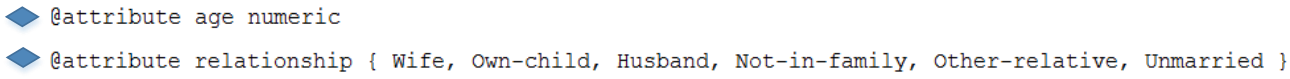
\includegraphics[width=5.5in]{chap4/attribute}
	\bicaption[fig4:attribute]{图}{连续和离散属性及其属性值}{Fig.}{numerical/categorical attribute and attribute value}
\end{figure}


\begin{figure}[!htp]
	\centering
	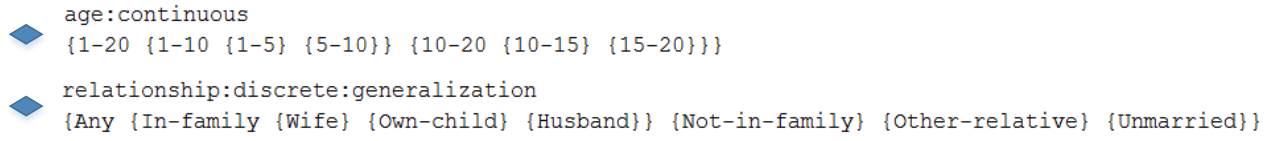
\includegraphics[width=5.5in]{chap4/semantic}
	\bicaption[fig4:semantic]{图}{属性的自定义匿名化结构语义}{Fig.}{The user-defined semantics of anonymous structure for attribute}
\end{figure}

DiffGen读取并解析匿名结构语义后,构建如图\ref{fig4:relationship}、图\ref{fig4:age}的匿名树,作为属性切割、数据集划分的依据。匿名树的叶节点用气泡框标识,也是最“细”的发布属性值。

\begin{figure}[!htp]
	\centering
	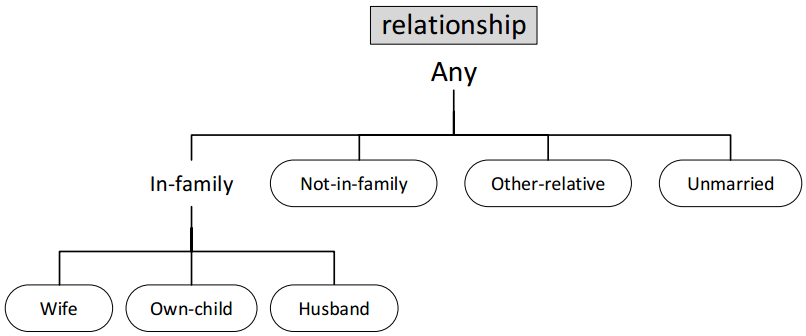
\includegraphics[width=5in]{chap4/relationship}
	\bicaption[fig4:relationship]{图}{根据属性relationship的匿名语义构建的匿名树}{Fig.}{A taxonomy tree for attribute relationship that is built by anonymous semantics}
\end{figure}

\begin{figure}[!htp]
	\centering
	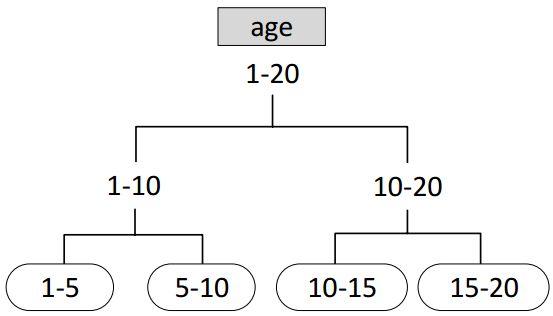
\includegraphics[width=3.5in]{chap4/age}
	\bicaption[fig4:age]{图}{根据属性age的匿名语义构建的匿名树}{Fig.}{A taxonomy tree for attribute age that is built by anonymous semantics}
\end{figure}

\subsection{算法框架}

在这个阶段,DiffGen算法依据匿名树的分裂规则,采用决策树算法通过指数机制逐层选择分裂属性,并作数据集划分,构建完整的分类树,最后在叶节点加噪并发布数据集。为了更清楚地展示这个过程以及理解DiffGen算法伪代码,继续使用前文公司应聘的例子做说明。
\begin{exmp}
	\label{chap4_exmp}
	某公司有8位应聘者,对属性“国籍”、“年龄”以及是否被成功录用做统计,类属性值的“是”、“否”表示为是否被录用。
\end{exmp}

图\ref{fig4:diffgen}展示了示例\ref{chap4_exmp}背景下的算法工作过程。算法\ref{diffgen}对DiffGen算法进行了完整描述,其中$Cut_{i}$表示在当分类树树高为i时,所有匿名树中可分裂的属性集合。如,仅有根节点时,$Cut_{1}$=\{亚洲,[15-40)\};而选取分裂属性亚洲后,$Cut_{2}$=\{东亚,西亚,[15-40)\}。$u(D,\cdotp)$表示打分函数,$S(u)$为其全局敏感性。


\begin{algorithm}
	\caption{DiffGen算法} 
	\label{diffgen}
	\begin{algorithmic}[1]
		\REQUIRE 隐私代价$\varepsilon$,树高$Hight$,数据集$D$。
		\ENSURE 新的匿名数据集$\hat{D}$。
		\STATE 初始化分类树根节点和$Cut_{i}$集合,此时i=1
		\STATE 按树高切割$\varepsilon$,统计连续属性个数为$A_{Pr}^{n}$,$\varepsilon$' $\leftarrow$ $\frac{\varepsilon}{2(|A_{Pr}^{n}|+2Hight)}$
		\STATE 对$Cut_{i}$里的每个连续属性$v_{n}$,计算其分裂点$p$,分裂点$p$的选中概率 $\wasypropto$ exp($\frac{\varepsilon\textasciiacute}{2S(u)}$$u(D,v_{n})$)
		\STATE 对所有的属性$v$, $\forall$$v$ $\in$ $Cut_{i}$,计算分值
		\FOR{i = 1 to $Hight$}
		\STATE 按分值选择属性$v$,$v$$\in$ $Cut_{i}$,且$v$的选中概率$\wasypropto$ exp($\frac{\varepsilon\textasciiacute}{2S(u)}$$u(D,v)$)
		\STATE 根据$v$的匿名树分裂节点$v$,$v$$\rightarrow$$child(v)$
		\STATE $Cut_{i}$ $\leftarrow$ $Cut_{i}$$ - $$v$,$Cut_{i}$ $\leftarrow$ $Cut_{i}$ $\cup$ $child(v)$
		\STATE 对$Cut_{i}$里的新出现的连续属性$v_{n}$,计算其分裂点$p$,分裂点$p$的选中概率 $\wasypropto$ exp($\frac{\varepsilon\textasciiacute}{2S(u)}$$u(D,v_{n})$)
		\STATE 对所有的属性$v$, $\forall$$v$ $\in$ $Cut_{i}$,更新分值
		\ENDFOR
		\RETURN 在叶子节点的数据项上,每个类属性计数为$C$,返回($C$+Laplace(1/$\varepsilon$))
	\end{algorithmic}
\end{algorithm}

在算法\ref{diffgen}中,选取分裂属性和处理连续属性分裂点时需要消耗隐私预算,因此在第2行对隐私预算进行了切分。在5-10行的每次迭代中,需要先对待选择属性集$Cut_{i}$的每个属性计算分值并对连续属性处理进行处理,然后通过指数机制按概率挑选属性。在第8行进行更新$Cut_{i}$集合操作,第9,10行更新分值。第12行在每个叶节点类属性计数上添加独立的拉普拉斯噪音,并返回。最后,在数据集发布阶段,根据类计数分布逐条发布匿名化数据集,如图\ref{fig4:diffgen}的下半部分所示。

\begin{figure}[!htp]
	\centering
	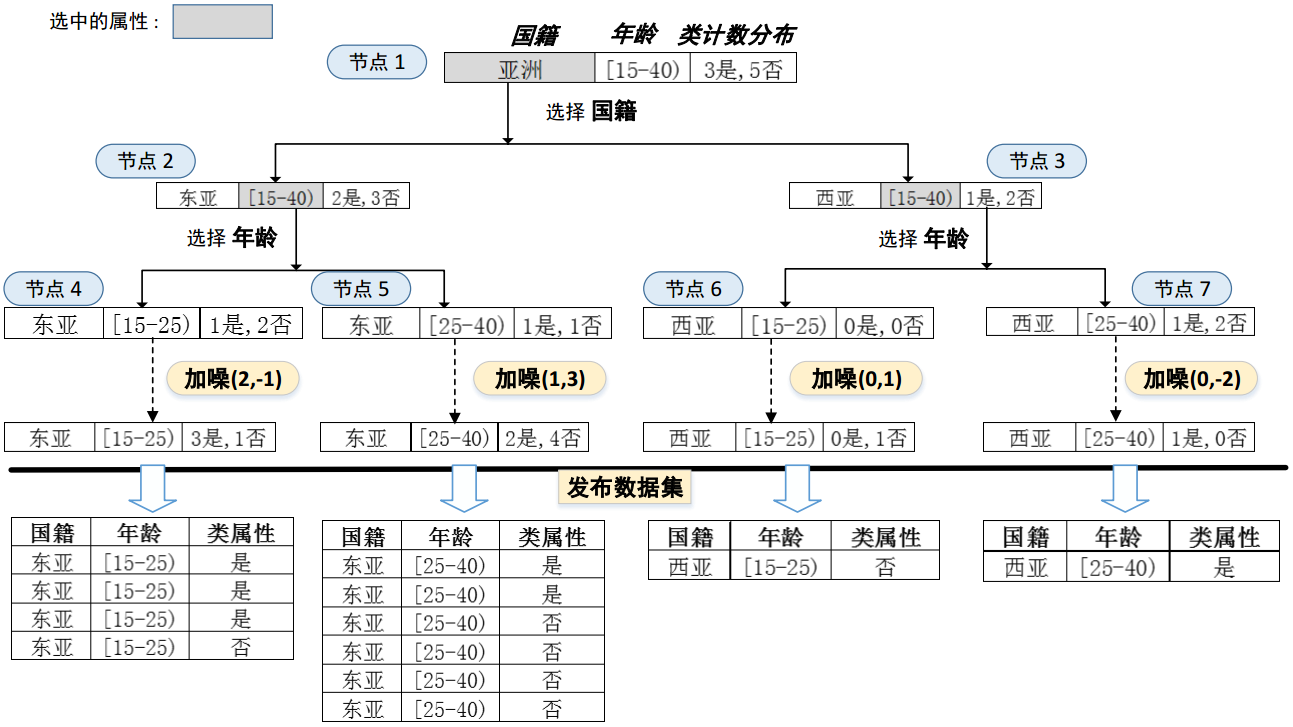
\includegraphics[width=6.2in]{chap4/diffgen}
	\bicaption[fig4:diffgen]{图}{DiffGen算法流程示例}{Fig.}{A sample for the procedure of DiffGen}
\end{figure}


\subsection{算法特性及模型启发}

基于前文对DiffGen算法的研究分析,本小节先总结了DiffGen数据发布模型所具有的相关性质,然后归纳其一致性特性以及与一维直方图发布方式间的联系,并给出相应证明。
\subsubsection{唯一性}
\begin{prop}
	\label{chap4_prop1}
	DiffGen分类树中,每个叶节点的属性值分布具有唯一性。
\end{prop}
\begin{proof}
	同\label{prop1}证明。
\end{proof}
此特性决定了针对某一属性范围的节点组合是非冗余的,保证了组合结果的唯一性。否则,冗余的查询结果会使得查询请求返回失败。

\subsubsection{完整性}

\begin{prop}
	\label{chap4_prop2}
	DiffGen分类树的构建过程中,每次属性的划分具有完整性,即对于某次分裂$v$$\rightarrow$$child(v)$,$child(v)$中的每个属性值在$Cut_{i}$中能够完整更新。
\end{prop}
\begin{proof}
	在DiffGen算法\ref{diffgen}的第7行,对挑选节点$v$的分裂操作是严格按照匿名树定义进行的。因此对于$\forall$ $cv$ $\in$ $child(v)$,必然有$cv$ $\in$ $Cut_{i}$。
\end{proof}

属性划分的完整性确保了合法查询请求的完整性,以下定义合法查询。

\begin{defn}
	(合法查询)有d个属性的数据集,属性$A_{i}$的匿名树上的所有属性值集合为$T_{i}$,$i$ $\in$ [1,d],则所有匿名树的属性值集合$T_{total}$ = $\sum\limits_i^d \cup T_{i}$。某查询请求$Q$涉及到$k$个不同的属性值查询,表示为$Q$=$\{a_{1},a_{2},...,a_{k}\}$,其中k $\leqslant$ |$T_{total}$|,$a_{k}$为属性值。若查询$Q$满足以下条件,则$Q$为合法查询:
	\begin{equation}
	\text{对于}\forall a_{i} \in Q, i \in [1,k], \text{总有}a_{i} \in T_{total}
	\end{equation}
	
\end{defn}


\begin{prop}
	\label{chap4_prop3}
	DiffGen发布的数据集使合法查询请求具有完整性,即对于合法查询请求中的任一属性值,均能在DiffGen分类树上找到应答节点。
\end{prop}
\begin{proof}
	设属性$A$的某一属性值$a$为某个合法查询请求中的查询属性值,且$A$的匿名树结构中$a$的父节点集合为$Fa$,$Fa$为根节点到$a$路径上的属性值集合。若$a$为根节点,即$a$=$Fa$,显然$a$就出现在分类树根节点上,应答节点即为根节点。若$a$$\neq$$Fa$,则$a$在分类树上有两种表现形式。(1)$a$在匿名树上的直接父节点属性值发生了分裂,由于\label{chap4_prop2}属性划分的完整性,则必然能在分类树上找到属性值为$a$的节点。(2)若$a$的间接父节点发生分裂或者属性$A$从未被选中,则在分类树上没有属性值为$a$的节点。但由于$a$$\in$$Fa$,那么在分类树中总能找到应答节点,它在$A$上的属性值为$Fa$中离$a$最近的父节点属性值,最坏情况下返回根节点作为应答。
	因此,对于合法查询请求中的任一属性值,在DiffGen分类树上总存在可覆盖此属性值的节点,保障所有查询项的完整性。
\end{proof}

\subsubsection{一致性}

\begin{prop}
	\label{chap4_prop4}
	在DiffGen分类树上,节点上的数据项之间具有一致性特性,可通过节点的组合运算应答合法查询请求。
\end{prop}
\begin{proof}
	叶节点上属性分布的唯一性保证了应答的正确性,匿名树和决策树算法的构建过程保证了严格的层级和泛化包含关系,结合\label{chap4_prop2}、\label{chap4_prop3}得证。
\end{proof}

一致性特性使得对于合法查询请求能够达到有求必应的效果,是DiffCon算法噪音优化算法和应答模式的基础。

\subsubsection{与一维直方图的联系} %正确性讨论,花了这么大力气一堆命题,就是为了说明可利用boost的思路

%最好能搞成命题啊1,范围覆盖,2相互独立(基于差分隐私组合性质)

基于相关的性质探讨,DiffGen的数据发布模型在范围查询需求中具有一维直方图的应答和组合特征。

一维直方图发布模型的特点在于能够响应所有的合法查询请求,对于属性值的范围查询能够通过一系列柱状条的叠加得到,并且单个柱状条计数值的增减改变是不影响其他柱状条的。而在多属性直方图中,随着属性值的增加使得数据集的数据域尺寸变大,若干个柱状条的叠加难以确保合法查询请求的完整性;并且,由于多属性的影响,每个柱状条之间不再相互独立。

在DiffGen模型中,虽然节点中的数据项包含多个属性,但叶节点构成的直方图不属于多属性直方图。合法查询请求的完整性解决了属性范围覆盖问题;分类树的一致性特性,使得对于所有属性范围的查询均可通过叶节点的组合给予应答,基于差分隐私的组合特性\cite{dpcombination},显然多属性分布的叶节点之间也是相互独立的。
在多维的类属性分布上,DiffGen模型看成是多个一维类属性直方图的组合,如例\ref{chap3_exmp},维护“已被录用”和“未被录用”两个类属性直方图即可。

因此本质上DiffGen模型具有一维直方图特征,此特征使得它和$BoostH$的基于一致性约束的优化方案具有相同的问题模型和理论基础,确保DiffCon优化算法中一致性约束设计的正确性。


\section{基于一致性约束的优化算法DiffCon}

针对范围计数查询应用,从基础算法出发,本节就基于一致性约束的优化思路,对非交互式差分隐私优化算法DiffCon的总体设计思进行详细阐述。主要分为以下几个部分:
\begin{enumerate}
	\item 立足于DiffGen的分类树结构,它是对原始数据集进行重匿名划分、生成新数据集的重要途径,是实施新的加噪方式的底层结构,是对外应答处理的算法基础。
	\item 改变基于数据条目的独立加噪和应答方式,重定义组合应答模式和全局敏感性。
	\item 设计并实现基于任意树结构的噪音调整算法,通过一致性约束优化噪音分布,使之更加合理。
	\item 基于分类树结构,对于范围查询可利用内部节点进行间接应答。展示DiffCon的组合应答模式及其处理算法。
\end{enumerate}

\subsection{辅助树结构}

DiffGen分类树是本课题优化算法的基础结构,噪音分布、优化技术以及查询应答原理均基于此。因此,以DiffGen的匿名树设计和分类树构建算法\ref{diffgen}为基础,DiffCon在生成分类树的同时维护辅助树形结构$DTree$。它可以看成是加噪、发布处理前分类树,但是额外维护了$LapNoise$和$OptNoise$两个变量,分别表示初始时的拉普拉斯噪音量和调整优化后的噪音量。定义$DTree$结构的伪代码如下,展示了其中的主要变量:

\begin{lstlisting}[language={C++}, caption={DTree结构伪代码}]
struct DTree{
	double $LapNoise$;
	double $OptNoise$;
	set<AttributePartition> $Cut_{i}$;
	vector<DTree*> children;
}
\end{lstlisting}
其中,"AttributePartition"为属性类型,$Cut_{i}$的意义与\ref{diffgen}算法中的一致,为所有匿名树中可分裂的属性集合。$DTree$结构对$Cut_{i}$的维护是为了保证分类树构建过程中,$DTree$节点与DiffGen分类树节点一一对应,确保树结构在分类过程中的正确性和完整性。

DiffCon算法的整体流程是基于DiffGen算法对数据集进行匿名化划分,生成完整的$DTree$树结构,然后对噪音分布进行调整,最后在叶节点上返回真实值和$OptNoise$的运算和。对比原算法\ref{diffgen}的返回值,第12行添加的噪音为叶节点的$LapNoise$,应替换为后置求精处理后的$OptNoise$。DiffCon算法的整体流程\ref{diffcon1}概括如下:

\begin{algorithm}
	\caption{DiffCon算法整体流程} 
	\label{diffcon1}
	\begin{algorithmic}[1]
		\REQUIRE 隐私代价$\varepsilon$,树高$Hight$,数据集$D$。
		\ENSURE 新的匿名数据集$\hat{D}$。
		\STATE 初始化分类树根节点、$Cut_{i}$集合,均分$\varepsilon$
		\STATE 初始化$DTree$的根节点$DTree_{R}$,并且$DTree_{R}->Cut_{i}$ $\leftarrow$ $Cut_{i}$
		\FOR{i = 1 to $Hight$,$DTree_{i}$表示$DTree$树的第i层节点集}
		\STATE 按DiffGen算法处理连续属性的分裂点,计算$Cut_{i}$中属性的分值并选出属性$v$,同时维护$Cut_{i}$
		\FOR{对于$DTree_{i}$中的每个节点$DTree_{node}$}
		\IF{$v$ $\in$ $DTree_{node}$->$Cut_{i}$} 
		\FOR{每个$cv$ $\in$ $child(v)$}
		\STATE 构建节点$Node_{cv}$,$Node_{cv}$->$Cut_{i}$ $\leftarrow$ $DTree_{node}$->$Cut_{i}$ $ - $ $v$ $\cup$ $cv$
		\STATE $DTree_{node}$->$children$ $\leftarrow$ $DTree_{node}$->$children$ $\cup$ $Node_{cv}$
		\ENDFOR
		\ENDIF 
		\ENDFOR
		\ENDFOR
		\STATE 对$DTree$的每个叶节点有,$LapNoise$ $\leftarrow$ Laplace($S(DiffCon)$/$\varepsilon$)
		\STATE 以$DTree$树结构为基础,运行优化算法DiffConOpt
		\RETURN 在叶子节点的数据项上,每个类属性计数为$C$,返回($C$+$OptNoise$))
	\end{algorithmic}
\end{algorithm} 

在算法\ref{diffcon1}中,属性的处理和选择均基于DiffGen算法,保证分类树和$DTree$树的同步构建。从第5行开始,对于挑选出的属性$v$,按照分裂$v$$\rightarrow$$child(v)$,为当前节点的构造子节点集。以此属性的匿名树为依据,有|$child(v)$|个属性则有|$child(v)$|个子节点,在第7行针对每个属性构建子节点,第8行更新节点的$Cut_{i}$域。第14行更新$LapNoise$变量,其中$S(DiffCon)$为重定义的全局敏感性,将在下一小节详细说明。在第15行运行优化算法DiffConOpt之后,$OptNoise$为优化后的噪音量,它将替代$LapNoise$在第16行与类计数的真实值做相加运算,最后返回并生成发布数据集。

\subsection{重定义应答模式和全局敏感性}
本小节将基于基础模型——直方图发布方式,对查询请求进行量化表述,讨论更改加噪模式前后的全局敏感性定义,并给出相关证明。

直方图的查询请求$mathcal{Q}$可以表示为一系列单位长度项的查询集合,根据前文讨论这也是DiffGen的应答模式。数据集的数据域尺寸为Domain,共有n个行项(柱状条),每个行项$x_{i}$(i$\in$[1,n])的计数值为$C(x_{i})$,那么有m个请求的查询序列$\mathcal{Q}$表示为
\[
	\mathcal{Q} = \{C(x_{1}),C(x_{2}),...,C(x_{m})\},m \in Domain,\|C(x_{2})\|_{1} = 1
\]

\begin{exmp}
	\label{chap4_exmp}
	直方图\ref{fig:histogram}的全属性查询为$\mathcal{Q}$ = $\{C([15-19]),C([20-24]),C([25-29],C([30-34]),C([35-40])\}$,且$\mathcal{Q}$ = \{1,2,3,0,2\}。
\end{exmp}

由全局敏感性的定义,

引出树的敏感性,小波和boost里边有,给出定义;研究下DiffGen的敏感性

给图说明新的应答模式

应说清 为了利用一致性进行应答,因此全局敏感要改,但是还是落在叶节点上。

\subsection{噪音调整算法}

\subsection{组合应答模式}

\subsection{流程总结}

\section{本章小结}